\documentclass{beamer}
\usepackage{graphicx}
\usetheme{Warsaw}
\title[]{EE1390}
\subtitle{Matrix Project}
\graphicspath{ {Home/Downloads/} }
\author{EE18BTECH11027 and EE18BTECH11011}
\date{}

\begin{document}


\begin{frame}
\titlepage
\end{frame}

\begin{frame}{Question}
Find the equation of the tangent to the circle,
at the point

\setlength{\parindent}{4cm}
$\binom{1}{-1}$
whose centre is the point of intersection of the
straight lines

\setlength{\parindent}{4cm} 
		(2 1)$\boldsymbol{x}-3=0$


		(1 -1)$\boldsymbol{x}-1=0$
		
\end{frame}		

\begin{frame}{Solution}
Given the equations of two lines:
\setlength{\parindent}{4cm}  

     
 (2 1)$\boldsymbol{x}-3=0$

		    (1 -1)$\boldsymbol{x}-1=0$
\setlength{\parindent}{0cm}

Solving these two equations , we get the point of intersection as I,which is the centre of the circle.
\vspace{2 mm}
\setlength{\parindent}{4cm}

$\binom{2 \ 1}{1  \  -1}$ $\boldsymbol{x}$ = $\binom{3}{1}$

\vspace{2 mm}
$\boldsymbol{x}$ =  $\binom{1/3 \  1/3}{1/3  \   -2/3}$ $\binom{3}{1}$

\vspace{2 mm}

$\boldsymbol{x}$ = $\binom{4/3}{1/3}$

\vspace{2 mm}
\setlength{\parindent}{0.5cm}

So coordinates of P in matrix form are $\binom{4/3}{1/3}$
\end{frame}


\begin{frame}


The radius of the circle is given by norm of $\binom{1}{-1}$ - 
$\binom{4/3}{1/3}$
which gives radius equal to $\sqrt{17/9}$.

now we find the tangent to the circle.

The directon vector of tangent is given by-
$\binom{1/3 \  1/3}{1/3  \   -2/3}$ $\binom{1}{-1}$ - 
$\binom{4/3}{1/3}$

which simplifies to $\binom{-4/3}{1/3}$


Equation of tangent is given by-
$\binom{1}{4}$ $\boldsymbol{x}$ = -3



\end{frame}
\begin{frame}
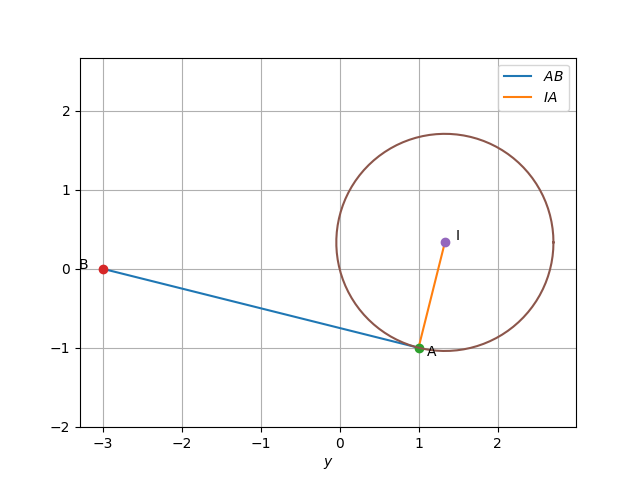
\includegraphics[scale=0.8]{../../Downloads/Figure_1(1).png}

\end{frame}
\end{document}


